	\newpage
\section{Ogólne określenie wymagań}		%1
%Ogólne określenie wymagań i zakresu programu (Czyli zleceniodawca określa wymagania programu) 
\begin{itemize}
	\item Aplikacja powinna korzystać z aktualnej lokalizacji użytkownika, a za pomocą Google Maps wyświetlać najbliższe sklepy spożywcze żabka.
	\begin{figure}[!hbt]
		\begin{center}
			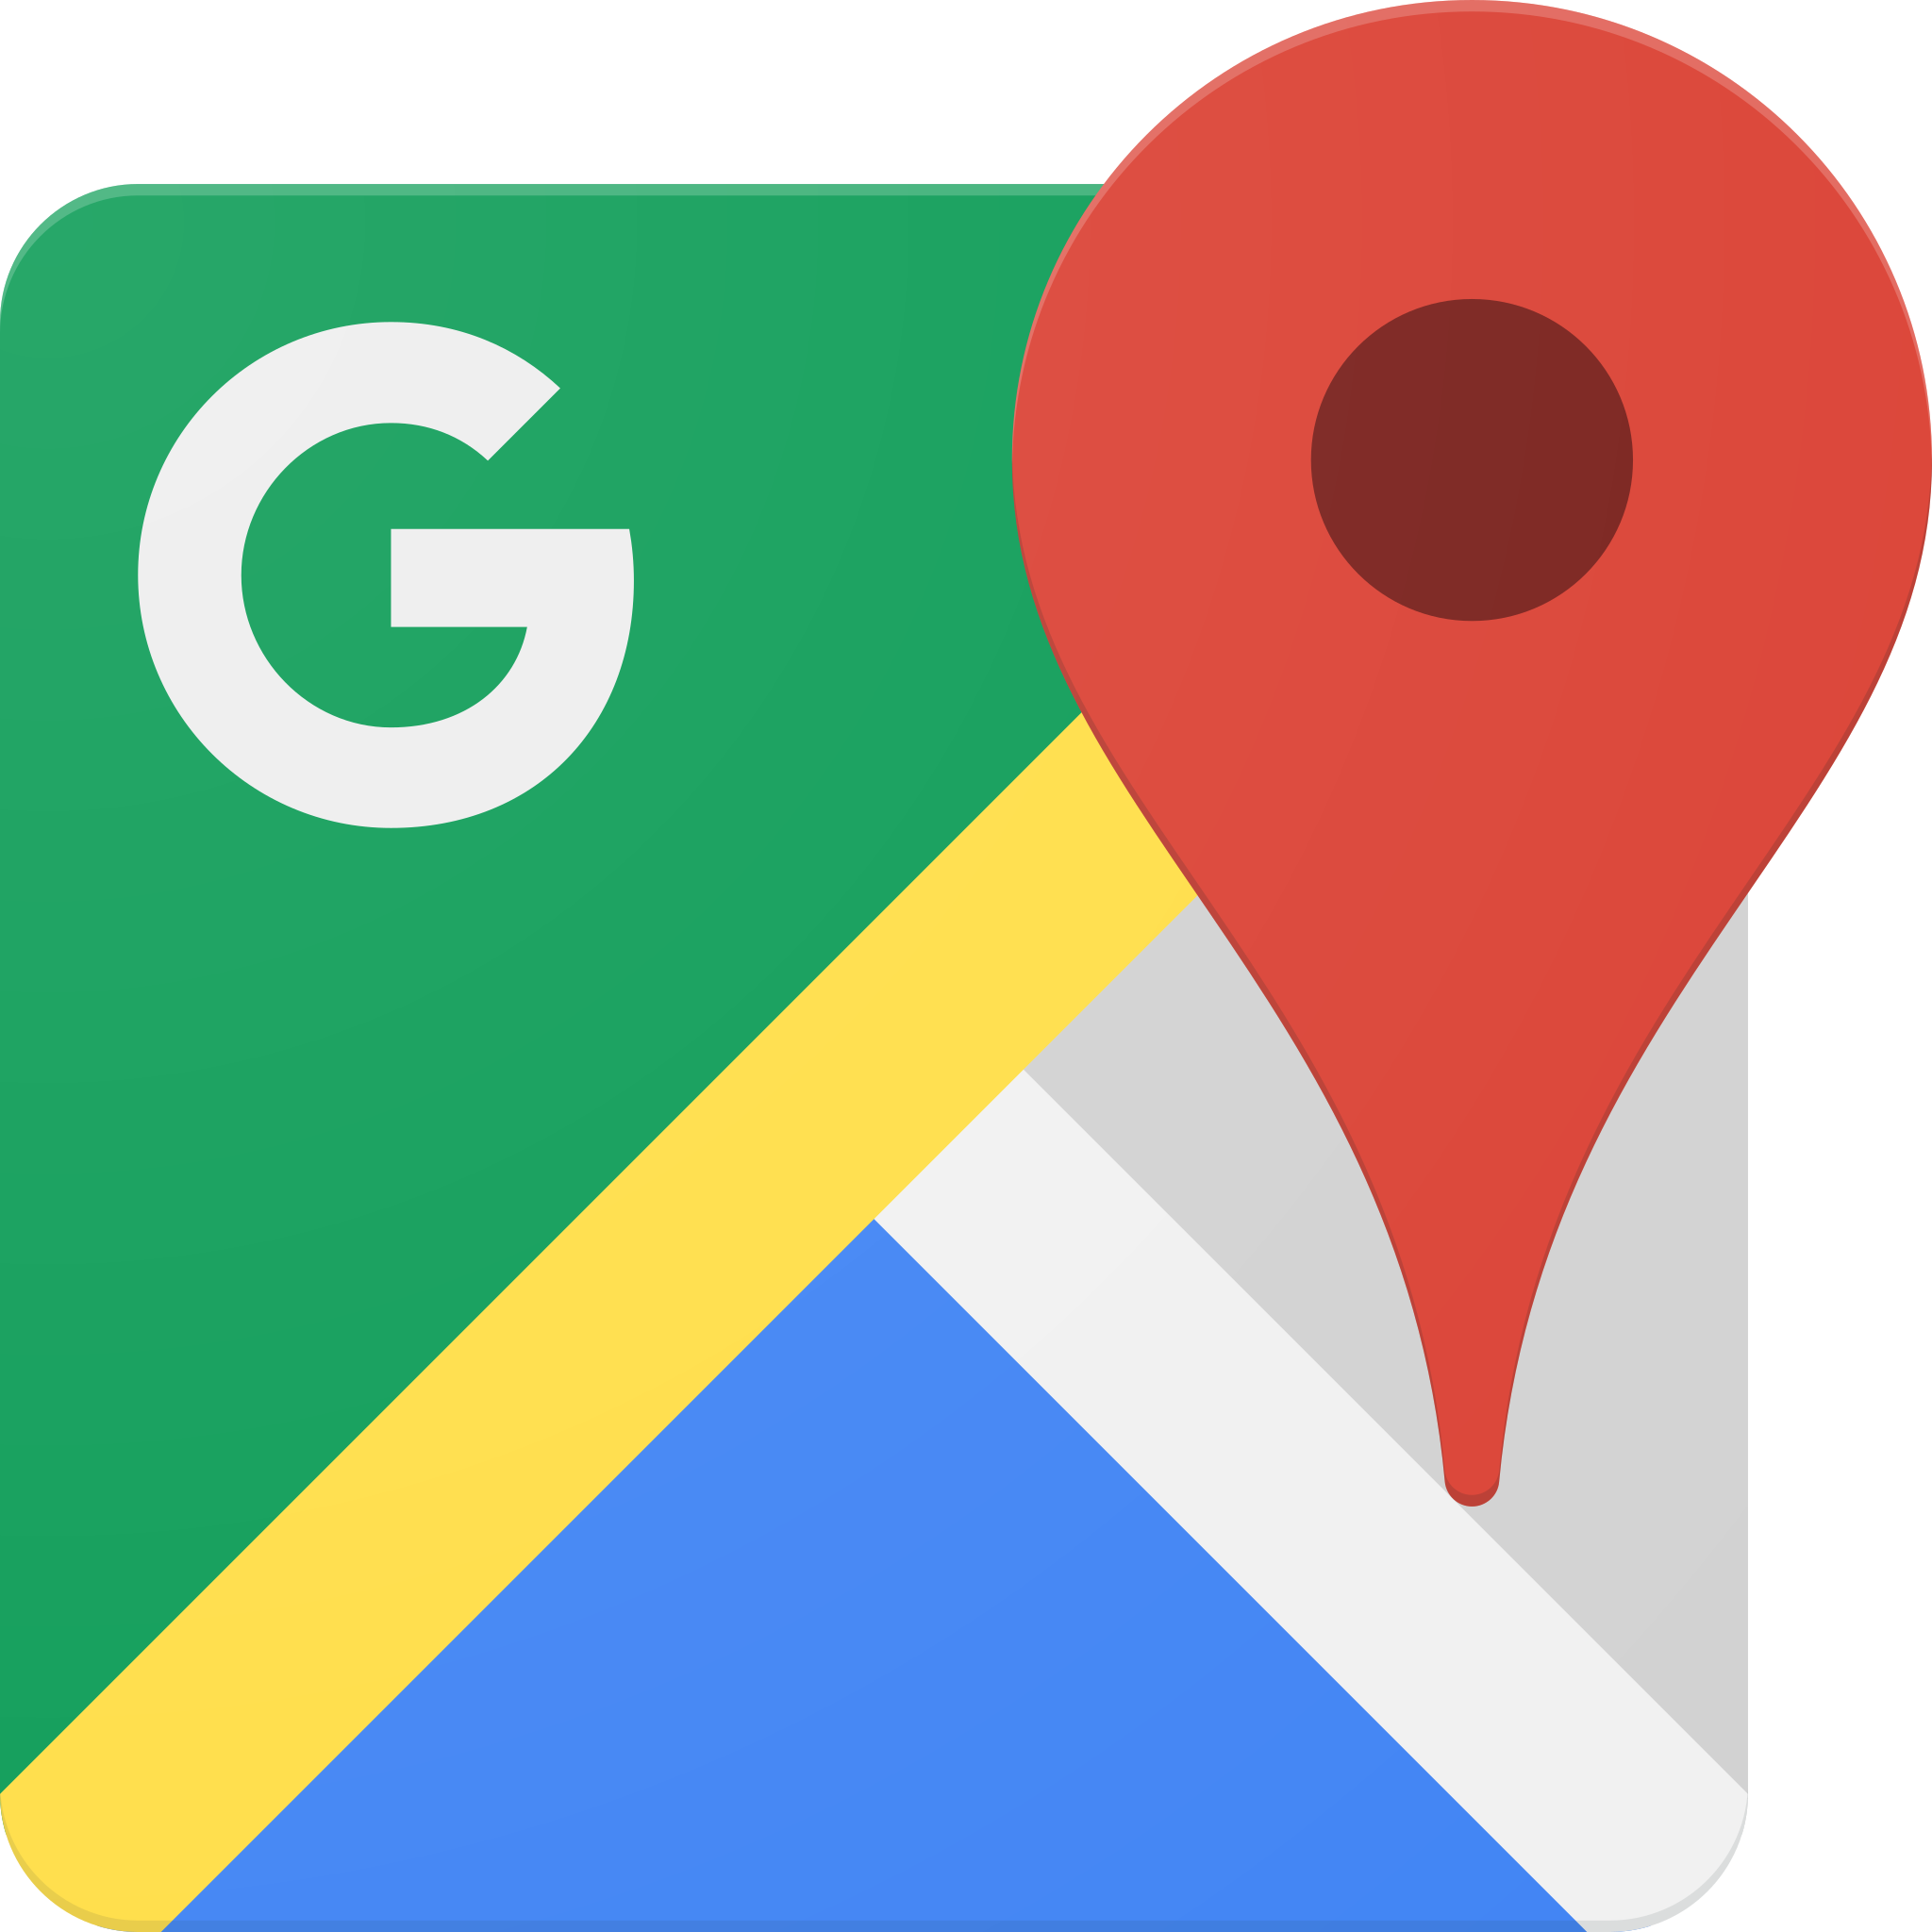
\includegraphics[width=6cm]{rys/Google-maps.png}
			\caption{Google maps}
			\label{rys:gps-icon}
		\end{center}
	\end{figure}
	\item Użytkownik powinien mieć możliwość wyświetlania sklepów spożywczych Żabka na mapach wraz z ich odległością od aktualnej lokalizacji.
	\item Aplikacja powinna umożliwiać użytkownikom przeglądanie szczegółów sklepów, takich jak godziny otwarcia, dostępne produkty i oceny klientów, po stronie Google Maps.
	\item Aplikacja umożliwia skanowanie kodów QR do sprawdzania najnowszych promocji i cen w sklepach Żabka.
	\item Klienci powinni mieć możliwość zaplanowania trasy do wybranego sklepu spożywczego za pomocą Google Maps.
	\item Aplikacja powinna wyświetlać informacje o dostępności produktów i cenach w poszczególnych sklepach spożywczych.
	\item Użytkownicy powinni mieć możliwość zapisywania ulubionych sklepów spożywczych i otrzymywania powiadomień o promocjach lub specjalnych ofertach.	
\end{itemize}